\documentclass[11pt,a4paper]{article}
\usepackage[T1]{fontenc}
\usepackage[utf8]{inputenc}
\usepackage{lmodern}
\usepackage[margin=22mm,headheight=16pt]{geometry}
\usepackage{amsmath,amssymb,graphicx,array,longtable,booktabs}
\usepackage{microtype,xcolor,hyperref,xurl,fancyhdr}
\definecolor{Navy}{HTML}{17324D}
\definecolor{Teal}{HTML}{087F8C}
\definecolor{Gold}{HTML}{B88128}
\hypersetup{colorlinks=true,linkcolor=Navy,urlcolor=Teal,bookmarksnumbered=true,hypertexnames=false}
\setlength{\parindent}{0pt}
\setlength{\parskip}{6pt}
\setlength{\emergencystretch}{4em}
\setcounter{tocdepth}{1}
\pagestyle{fancy}\fancyhf{}
\fancyfoot[R]{\small\thepage}
\fancyfoot[L]{\small\sffamily Sharif University of Technology}
\renewcommand{\headrulewidth}{0.3pt}
\makeatletter
\renewcommand\section{\@startsection{section}{1}{\z@}{-3.2ex plus -1ex minus -.2ex}{1.6ex plus .2ex}{\normalfont\Large\sffamily\bfseries\color{Navy}}}
\renewcommand\subsection{\@startsection{subsection}{2}{\z@}{-2.5ex plus -1ex minus -.2ex}{1.2ex plus .2ex}{\normalfont\large\sffamily\bfseries\color{Teal}}}
\makeatother
\fancyhead[L]{\small\sffamily\color{Navy}Reza Sanaee Nezhad}\fancyhead[R]{\small\sffamily\color{Teal}Technical Report}\begin{document}
\begin{titlepage}\centering\vspace*{7mm}

\includegraphics[width=31mm]{assets/sharif_emblem_en.png}\par\vspace{5mm}
{\Large\sffamily\bfseries\color{Navy}SHARIF UNIVERSITY OF TECHNOLOGY\par}
\vspace{2mm}{\sffamily Department of Electrical Engineering\par}
\vspace{17mm}{\color{Teal}\rule{\linewidth}{1.4pt}}\par\vspace{6mm}
{\large\sffamily\color{Teal}TECHNICAL REPORT\par}
\vspace{8mm}{\huge\sffamily\bfseries\color{Navy}Large-Scale Traffic Pattern Mining and Detection-Consistency Analysis\par}
\vspace{9mm}{\color{Gold}\rule{45mm}{1pt}}\par\vfill
\begin{minipage}{.88\linewidth}{\sffamily\color{Teal}AUTHOR}\par{\Large\sffamily Reza Sanaee Nezhad}\par Student ID: 401101502\par\vspace{7mm}
{\sffamily\color{Teal}INSTRUCTOR / INSTRUCTORS}\par
Dr Iman Gholampour\par\vspace{7mm}
{\sffamily\color{Teal}ACADEMIC CONTEXT}\par
Big Data Processing\par\end{minipage}\vfill
\end{titlepage}
\tableofcontents\clearpage
\section{Data preparation and access experiment}

The dataset contains 32,769,490 recorded rows. The submission repartitions by PlateValue, sorts within partitions by event\_\allowbreak{}ts, and writes Parquet. This is a Spark data-layout optimization, rather than a classic B-tree index. The distinction matters because it is a documented deviation from the assignment's indexing method. The report compares a plate-filter operation on CSV at 63.78 seconds with the prepared Parquet path at 7.50 seconds. Their quotient is approximately 8.50;\allowbreak{} one other recorded timing comparison gives approximately 8.42, which must be labeled with its own observations. Differences include encoding, columnar scans, cached/\allowbreak{}warm execution, and layout, so the result cannot be attributed solely to an index. Parquet statistics and predicate pushdown can help skip data, but a hash repartition does not by itself guarantee direct file routing for every plate predicate. The actual plan and scan metrics should establish that mechanism. Filters on unrelated columns and broad aggregates can still require extensive reads. Even then, column pruning/\allowbreak{}compression can help, so claiming that every non-key query receives no benefit is too absolute. The retained source output shows the measured comparison without treating it as a universal speedup.

\begin{figure}[!htbp]\centering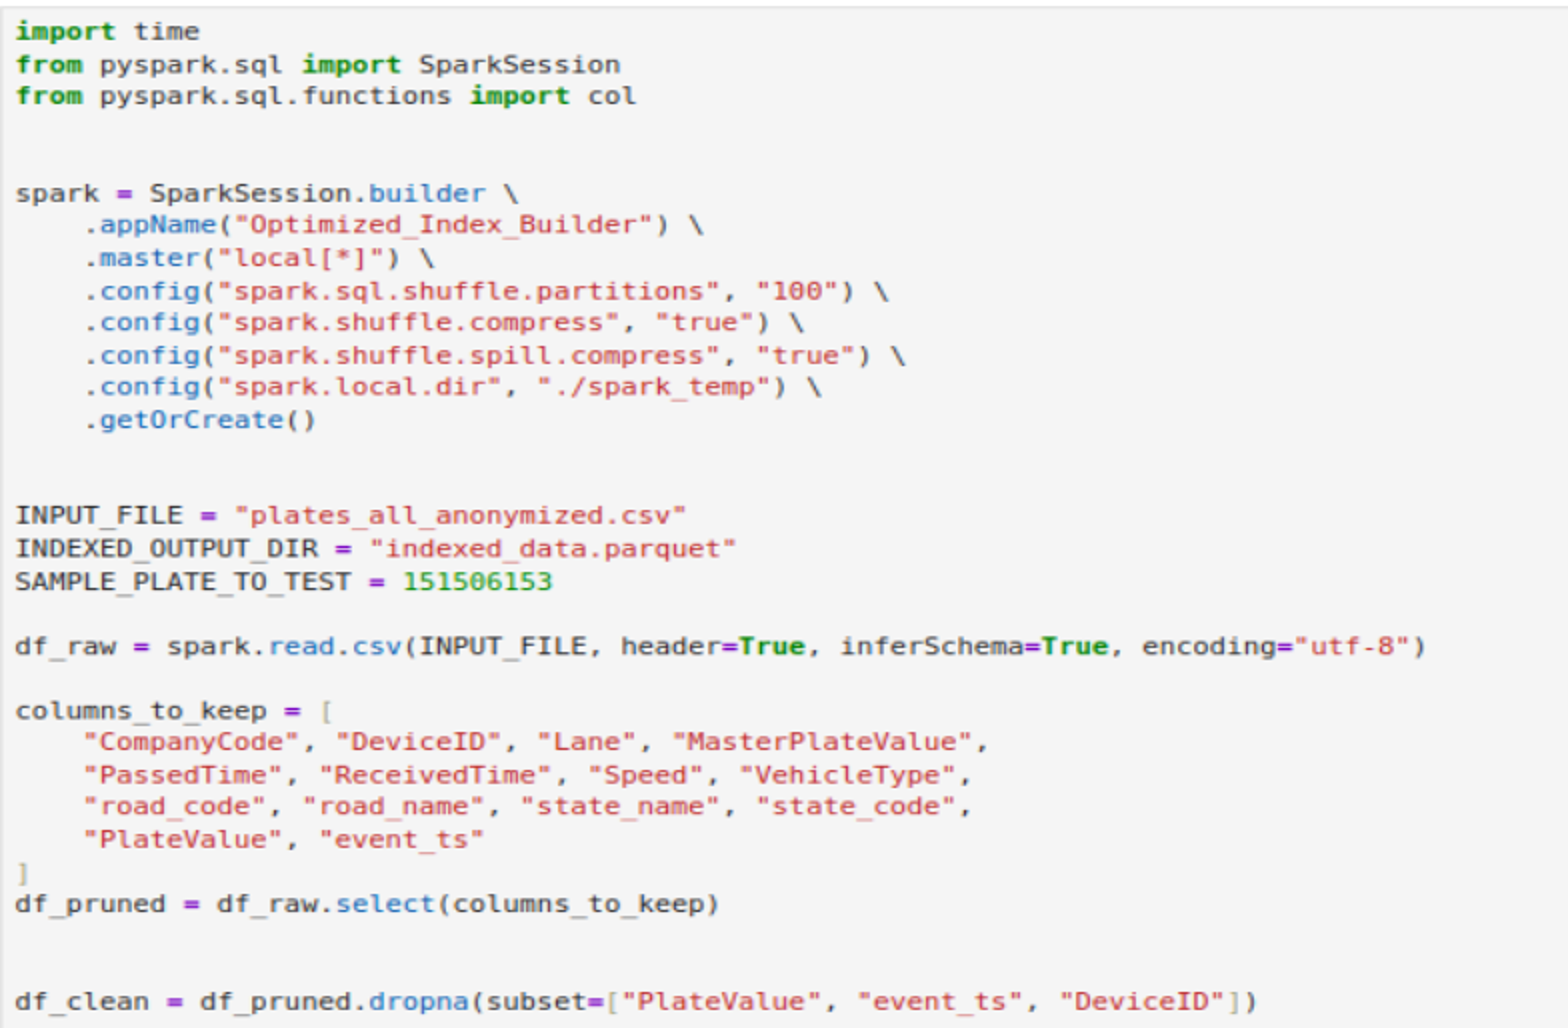
\includegraphics[width=\linewidth,height=.72\textheight,keepaspectratio]{assets/030_p001_01.png}\caption{Implementation and output: Data preparation and access experiment.}\label{fig:030_p001_010}\end{figure}
\begin{figure}[!htbp]\centering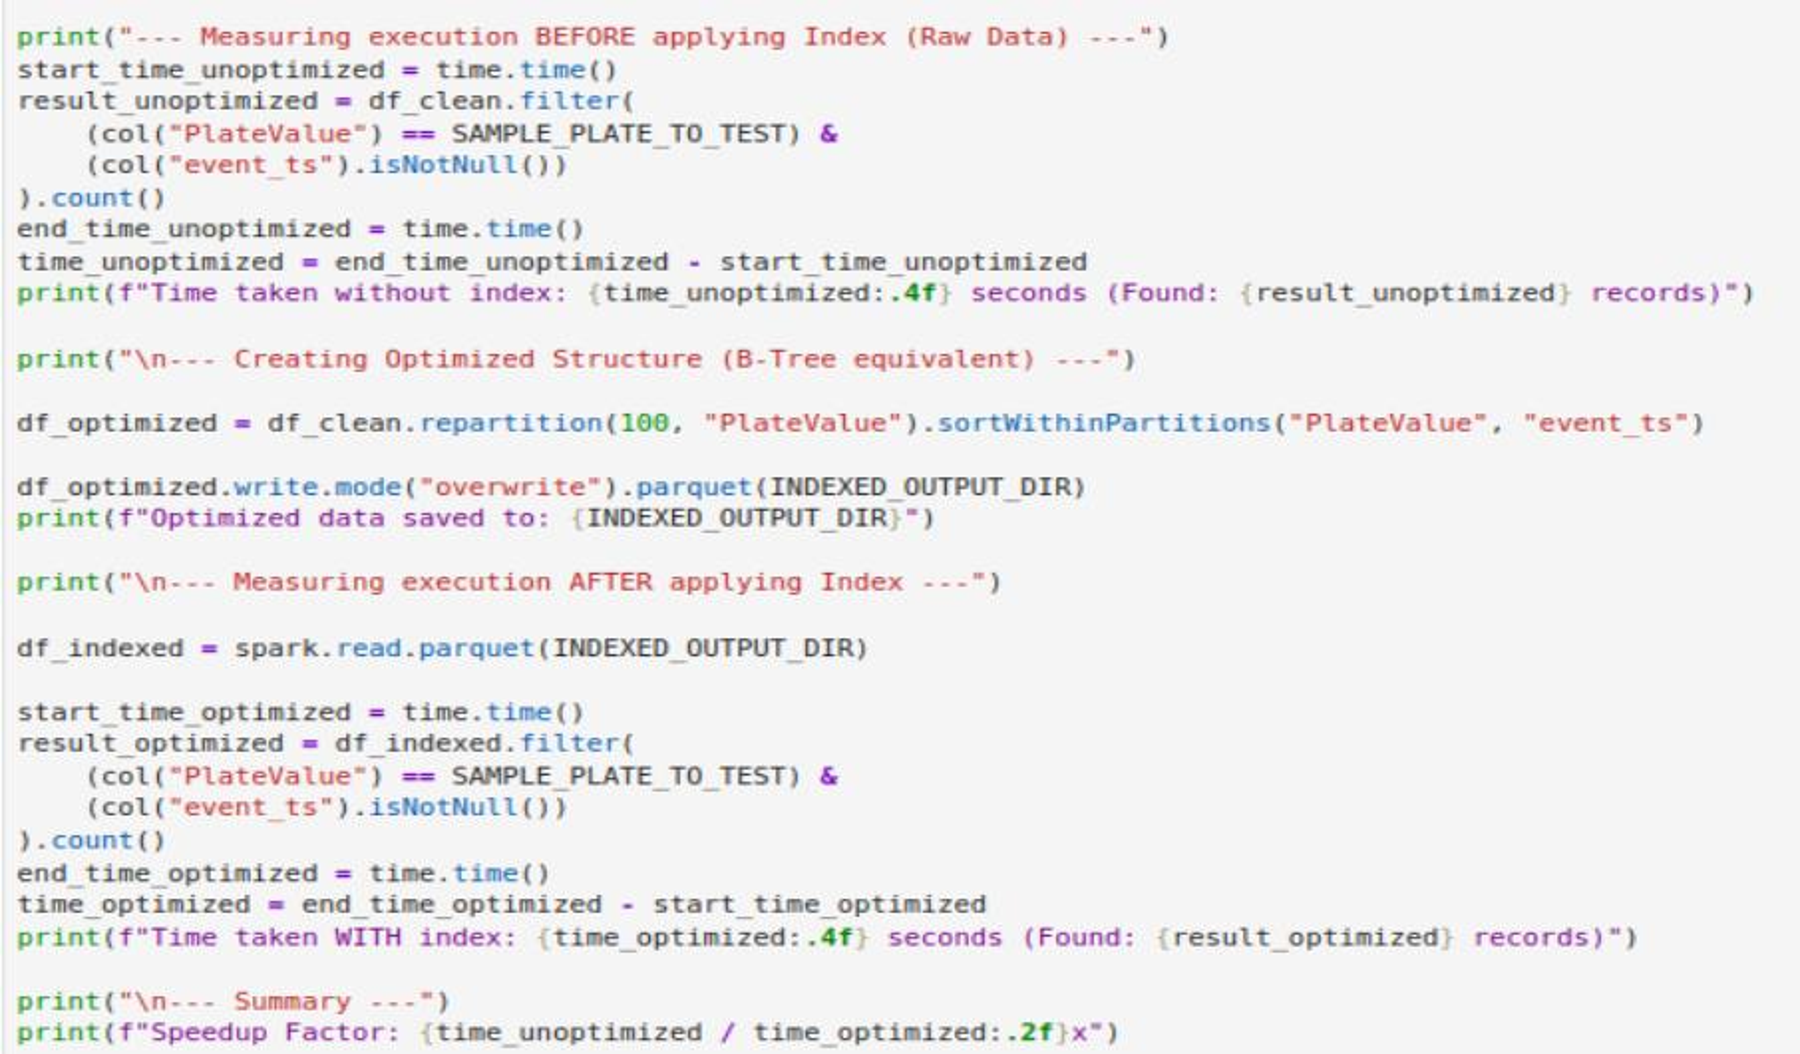
\includegraphics[width=\linewidth,height=.72\textheight,keepaspectratio]{assets/030_p001_02.png}\caption{Implementation and output: Data preparation and access experiment.}\label{fig:030_p001_020}\end{figure}
\begin{figure}[!htbp]\centering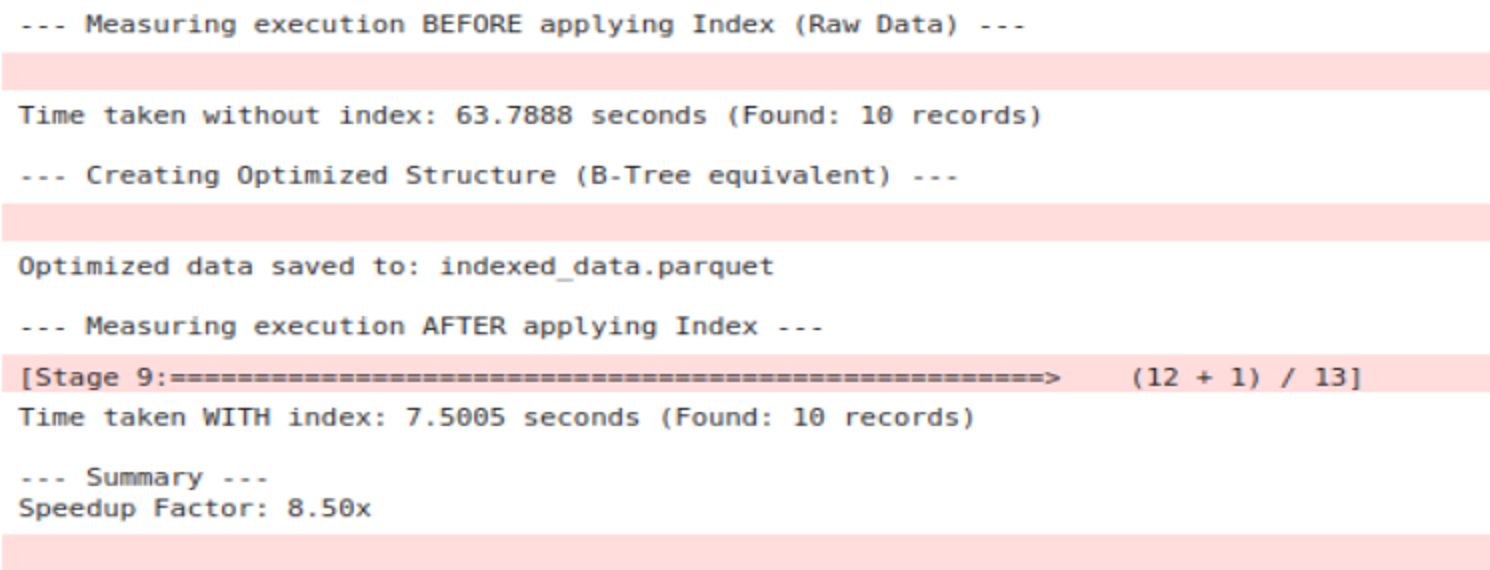
\includegraphics[width=\linewidth,height=.72\textheight,keepaspectratio]{assets/030_p002_01.png}\caption{Diagram or recorded result: Data preparation and access experiment.}\label{fig:030_p002_010}\end{figure}
\clearpage
\section{Market baskets and time-window sensitivity}

Each basket identifies a vehicle and a fixed event-time window. Items combine contractor and camera as CompanyCode\_\allowbreak{}DeviceID. Sets collapse repeated sightings of the same item;\allowbreak{} a three-item basket means at least three distinct items, not merely three rows. The report compares 30-minute and one-hour windows. The printed narrative describes roughly 28.6 million and 26.4 million initial baskets, with retained triple-capable fractions approximately 1.75 percent (about half a million) and 4.15 percent (about 1.09 million), respectively. The one-hour choice retains more co-occurrences in this observation and was selected for subsequent mining. It is not proved universally optimal, and fixed-window boundaries can split a real trip regardless of duration. The small plate-like value 5 appears in unusually large geographically scattered baskets. It may represent a default/\allowbreak{}unreadable identifier or another data-quality issue, but its meaning requires the dataset's encoding contract. Retaining such shared placeholders can create artificial high-support patterns, so the cleaning rule and effect on results must be explicit.

\begin{figure}[!htbp]\centering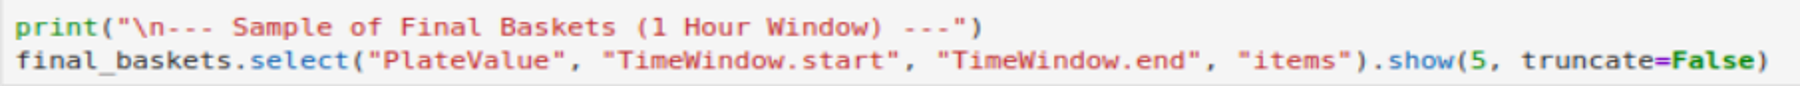
\includegraphics[width=\linewidth,height=.72\textheight,keepaspectratio]{assets/030_p004_01.png}\caption{Implementation and output: Market baskets and time-window sensitivity.}\label{fig:030_p004_010}\end{figure}
\begin{figure}[!htbp]\centering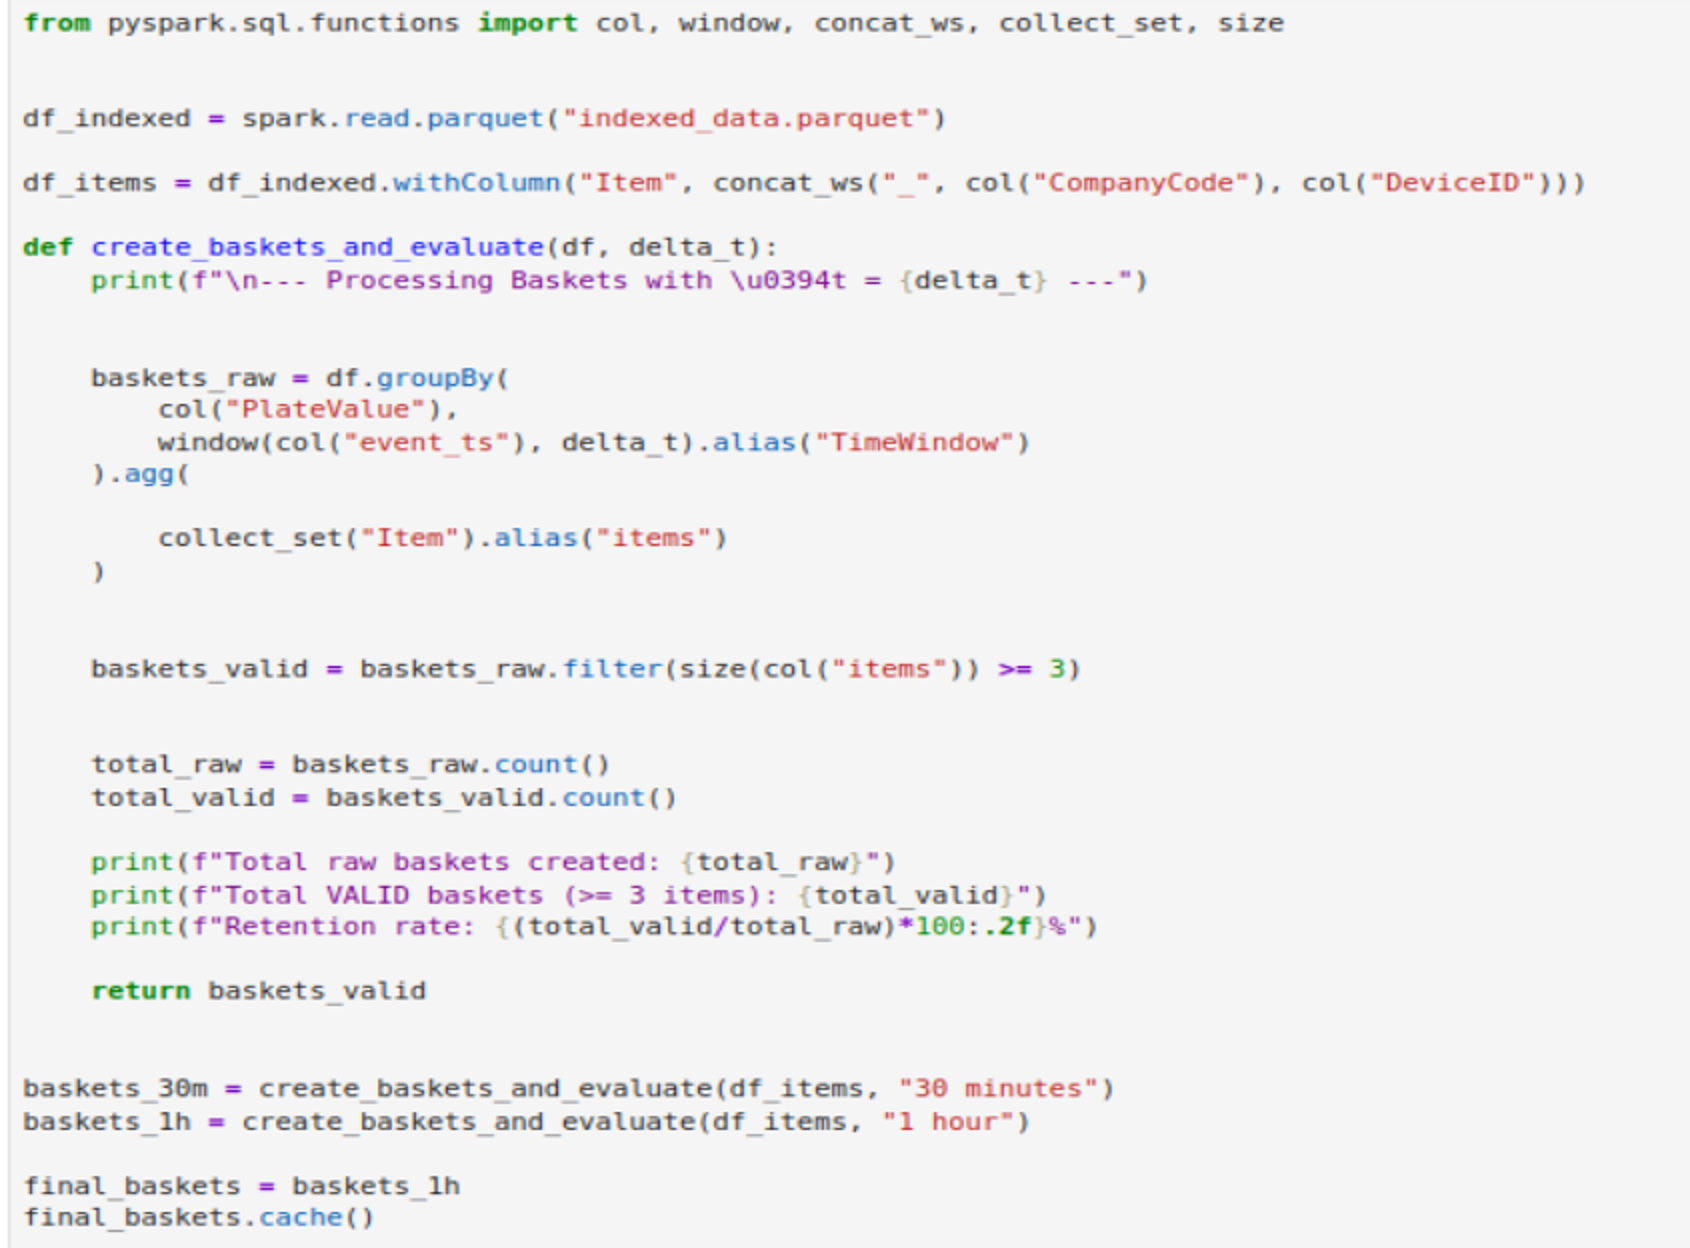
\includegraphics[width=\linewidth,height=.72\textheight,keepaspectratio]{assets/030_p004_02.png}\caption{Implementation and output: Market baskets and time-window sensitivity.}\label{fig:030_p004_020}\end{figure}
\begin{figure}[!htbp]\centering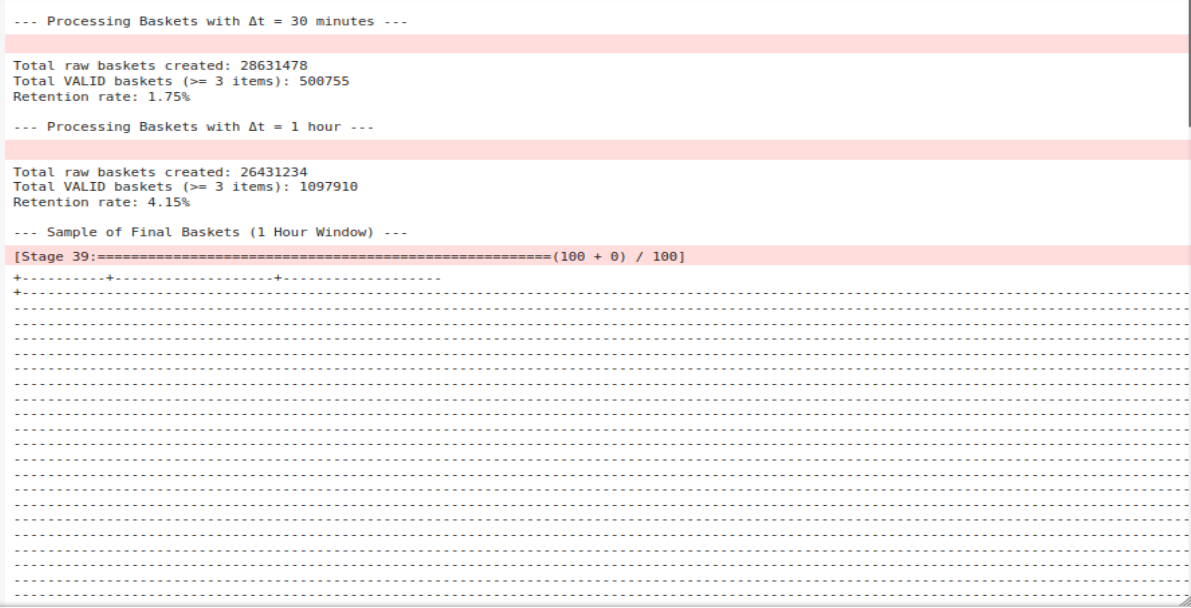
\includegraphics[width=\linewidth,height=.72\textheight,keepaspectratio]{assets/030_p004_03.png}\caption{Diagram or recorded result: Market baskets and time-window sensitivity.}\label{fig:030_p004_030}\end{figure}
\begin{figure}[!htbp]\centering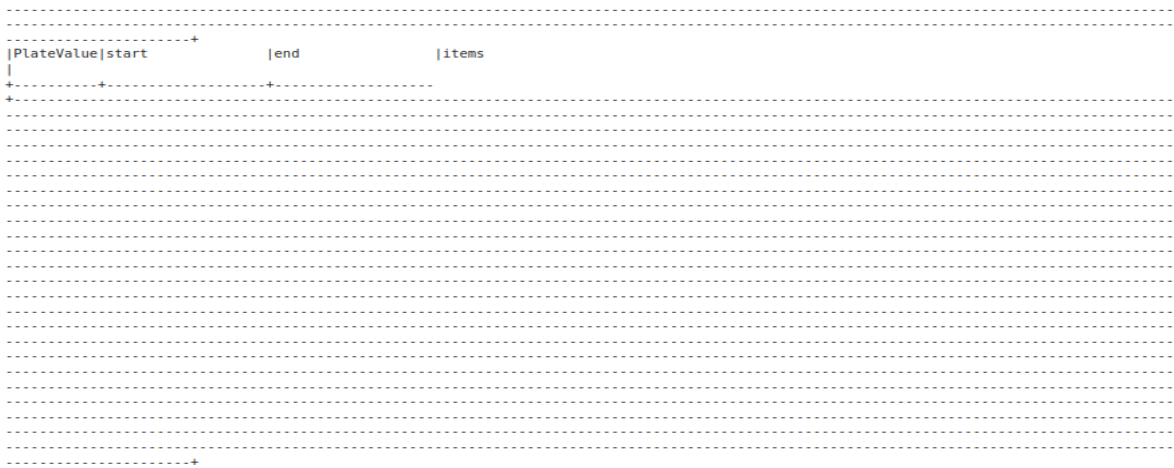
\includegraphics[width=\linewidth,height=.72\textheight,keepaspectratio]{assets/030_p005_01.png}\caption{Diagram or recorded result: Market baskets and time-window sensitivity.}\label{fig:030_p005_010}\end{figure}
\begin{figure}[!htbp]\centering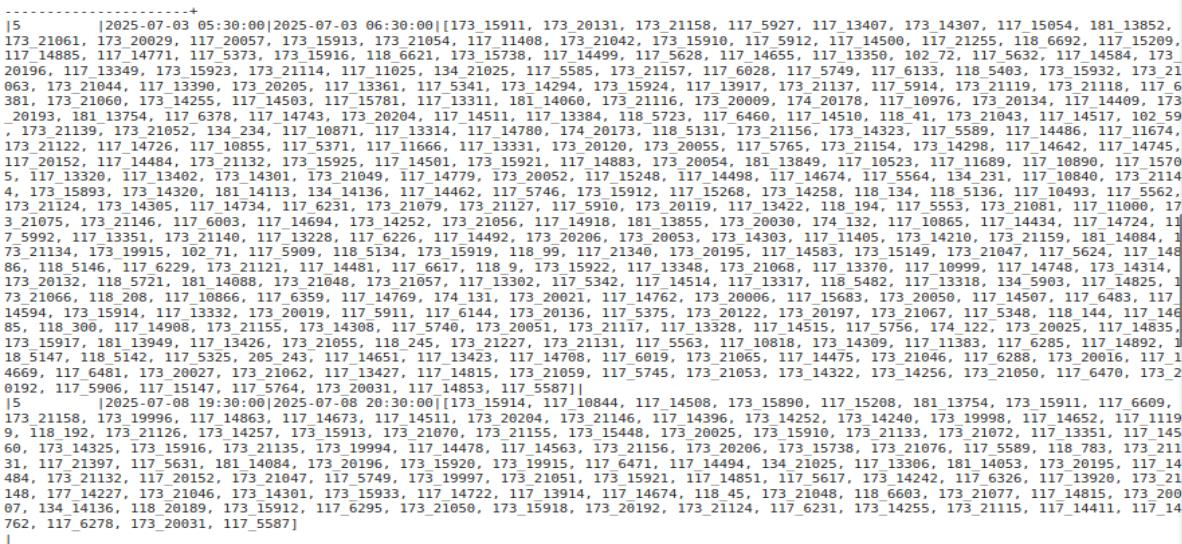
\includegraphics[width=\linewidth,height=.72\textheight,keepaspectratio]{assets/030_p005_02.png}\caption{Diagram or recorded result: Market baskets and time-window sensitivity.}\label{fig:030_p005_020}\end{figure}
\begin{figure}[!htbp]\centering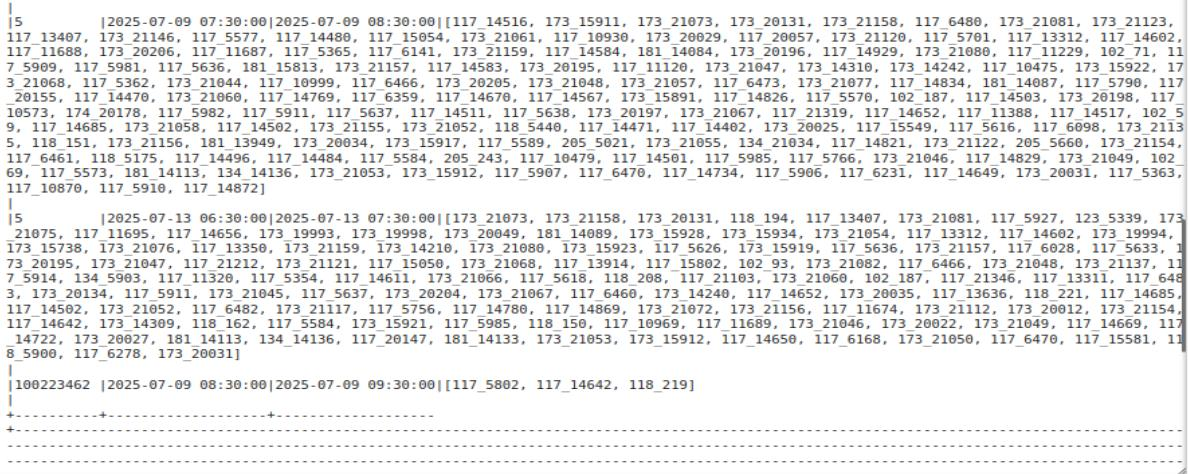
\includegraphics[width=\linewidth,height=.72\textheight,keepaspectratio]{assets/030_p005_03.png}\caption{Diagram or recorded result: Market baskets and time-window sensitivity.}\label{fig:030_p005_030}\end{figure}
\clearpage
\section{Frequent triples and algorithm choice}

The submission uses Spark FP-Growth with minSupport=\allowbreak{}0.001, equivalent to 0.1 percent of the supplied baskets. The assignment requested Apriori or PCY;\allowbreak{} FP-Growth is a methodological substitution. Explain it as the actual submitted algorithm, rather than relabeling it to meet the requirement. Support counts baskets. The same vehicle can contribute several baskets, so a threshold near a thousand supporting baskets is not necessarily a thousand distinct vehicles. A frequent unordered triple does not prove A-to-B-to-C order, physical adjacency, or a mandatory corridor. The report observes repeated contractor codes such as 123 and 117 within high-support triples, suggesting a pattern worth checking against camera placement/\allowbreak{}contract data. It does not establish exact operator territory from co-occurrence alone.

\begin{figure}[!htbp]\centering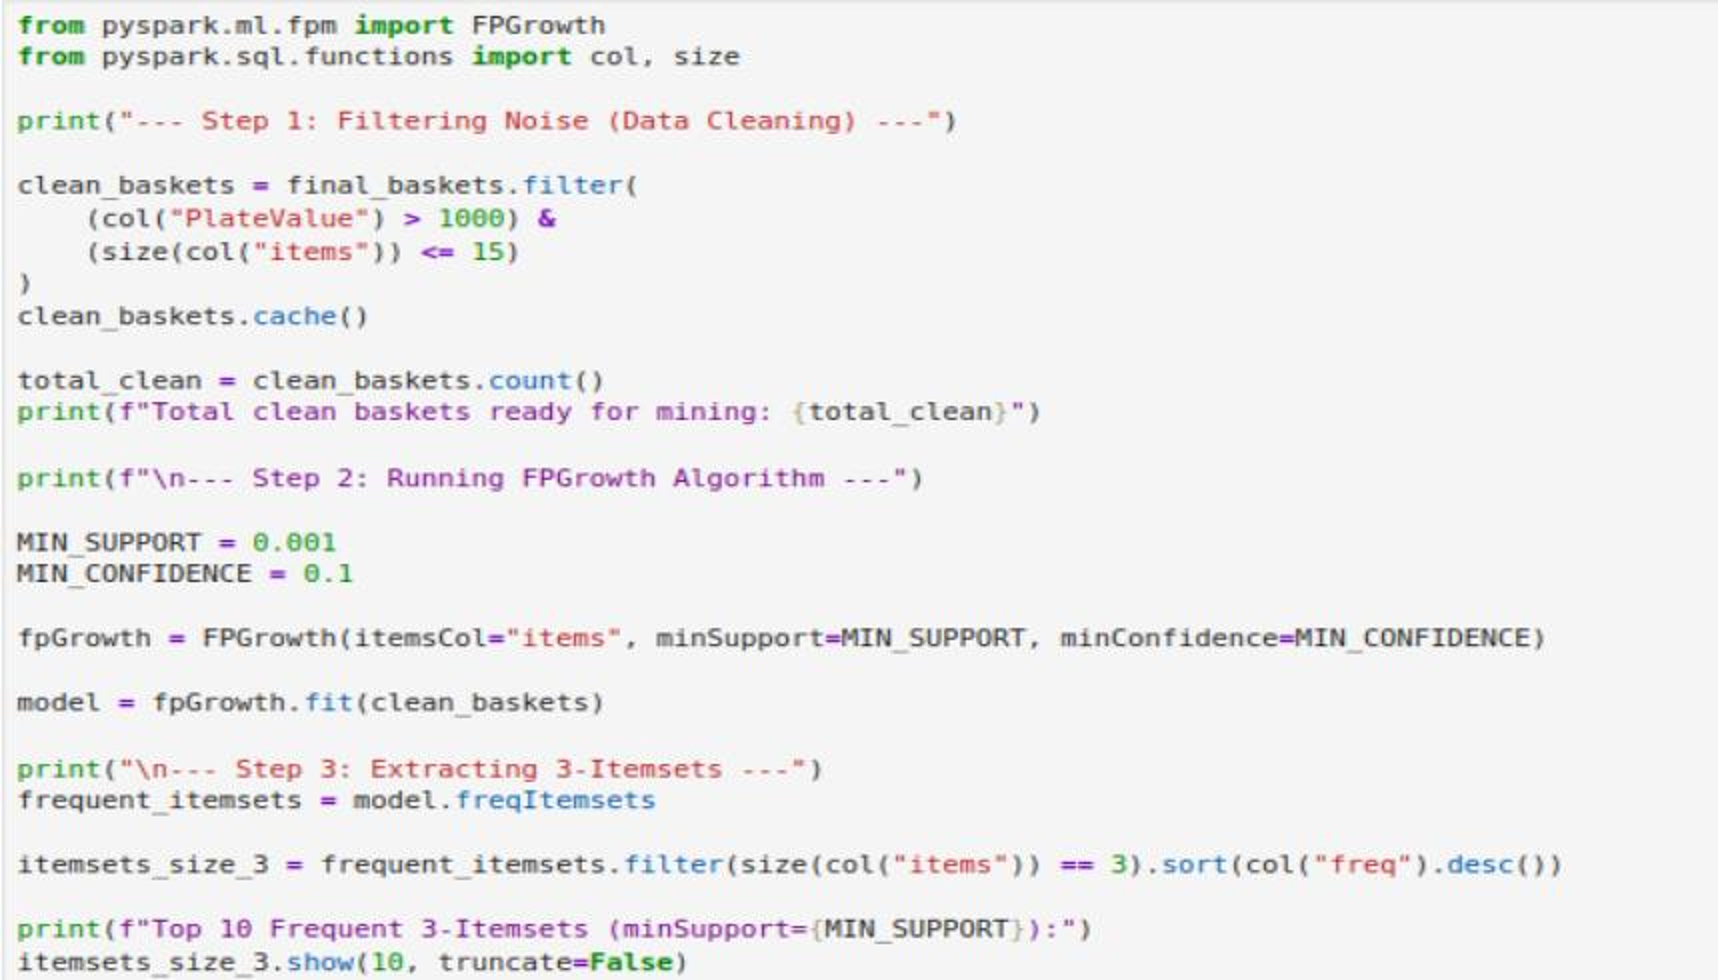
\includegraphics[width=\linewidth,height=.72\textheight,keepaspectratio]{assets/030_p008_01.png}\caption{Implementation and output: Frequent triples and algorithm choice.}\label{fig:030_p008_010}\end{figure}
\begin{figure}[!htbp]\centering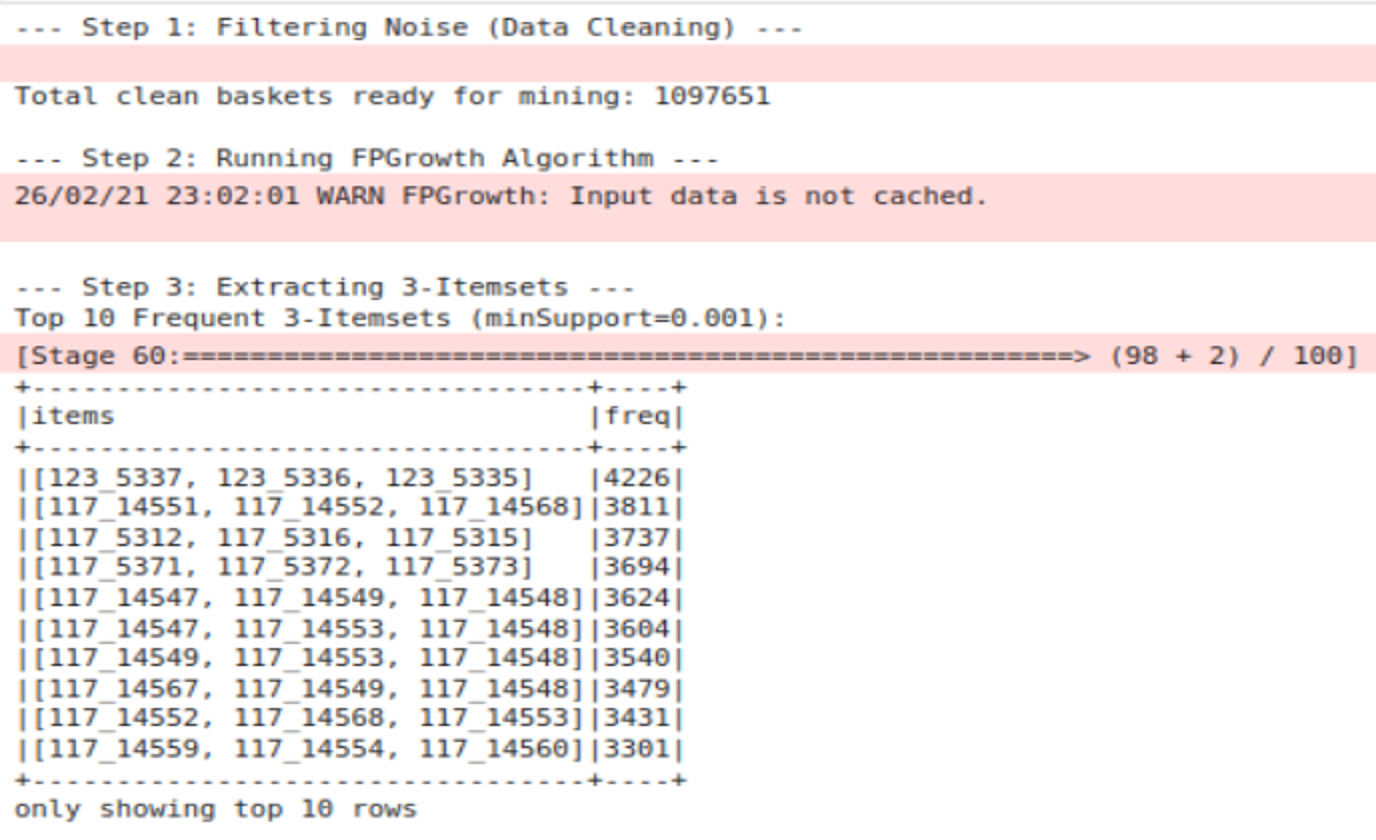
\includegraphics[width=\linewidth,height=.72\textheight,keepaspectratio]{assets/030_p008_02.png}\caption{Diagram or recorded result: Frequent triples and algorithm choice.}\label{fig:030_p008_020}\end{figure}
\begin{figure}[!htbp]\centering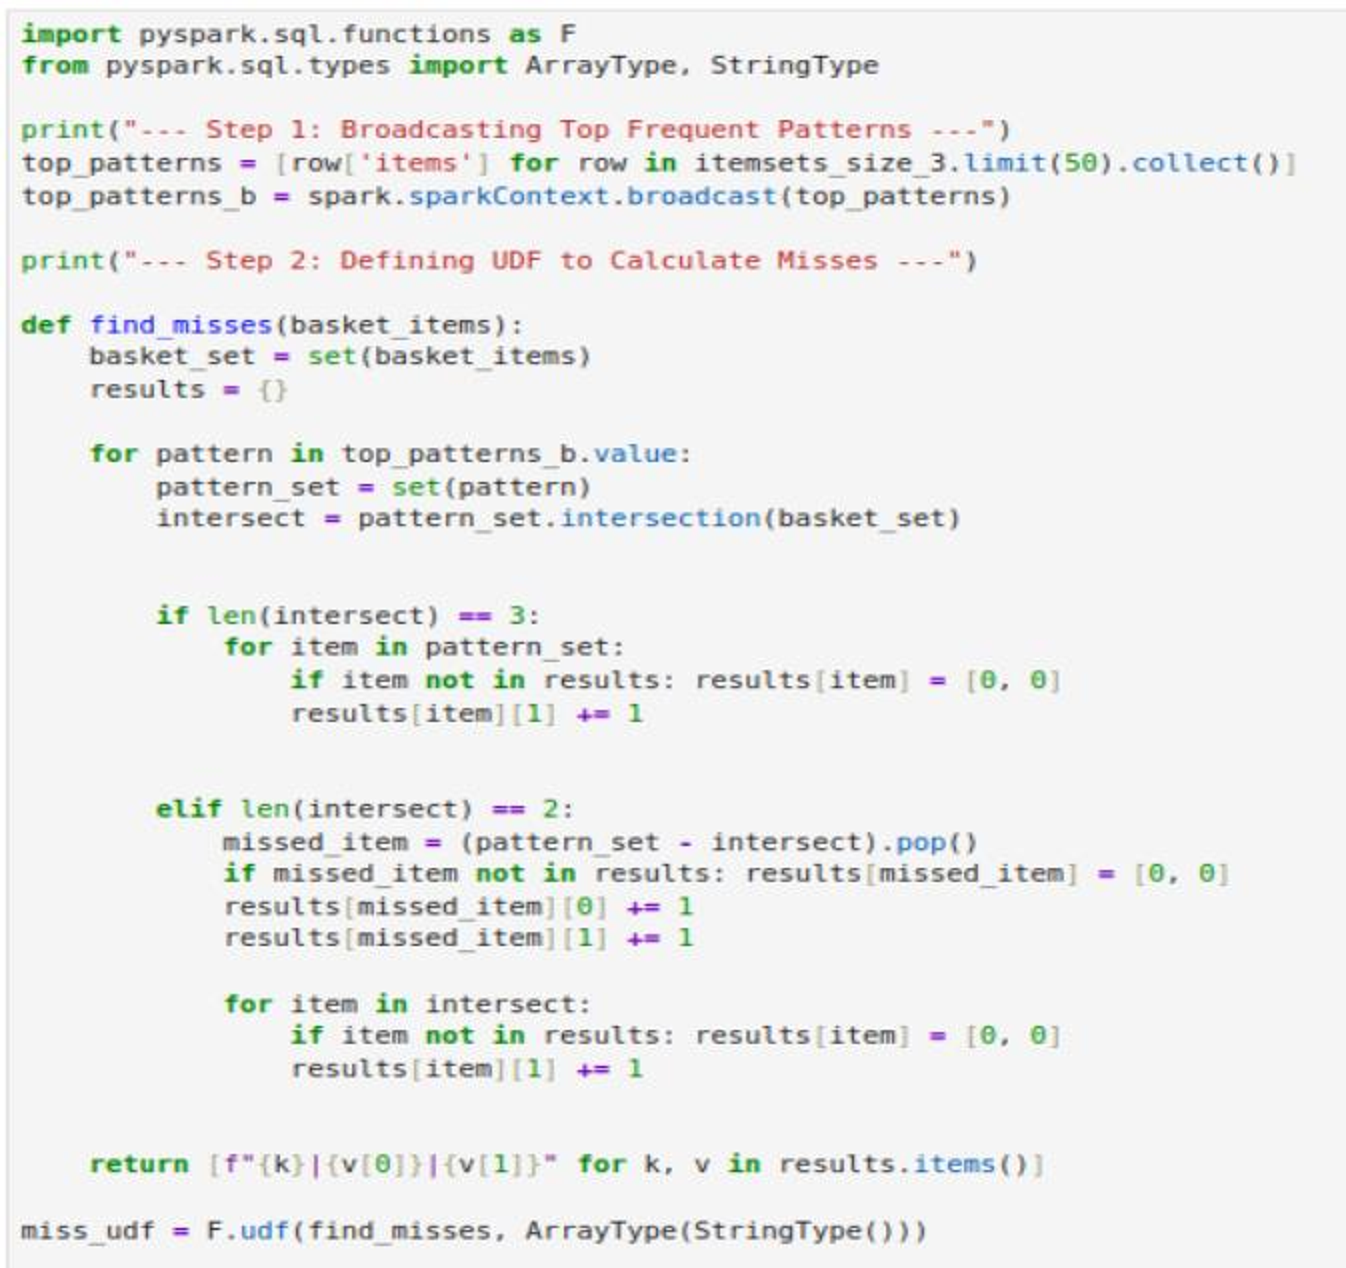
\includegraphics[width=\linewidth,height=.72\textheight,keepaspectratio]{assets/030_p010_01.png}\caption{Implementation and output: Frequent triples and algorithm choice.}\label{fig:030_p010_010}\end{figure}
\begin{figure}[!htbp]\centering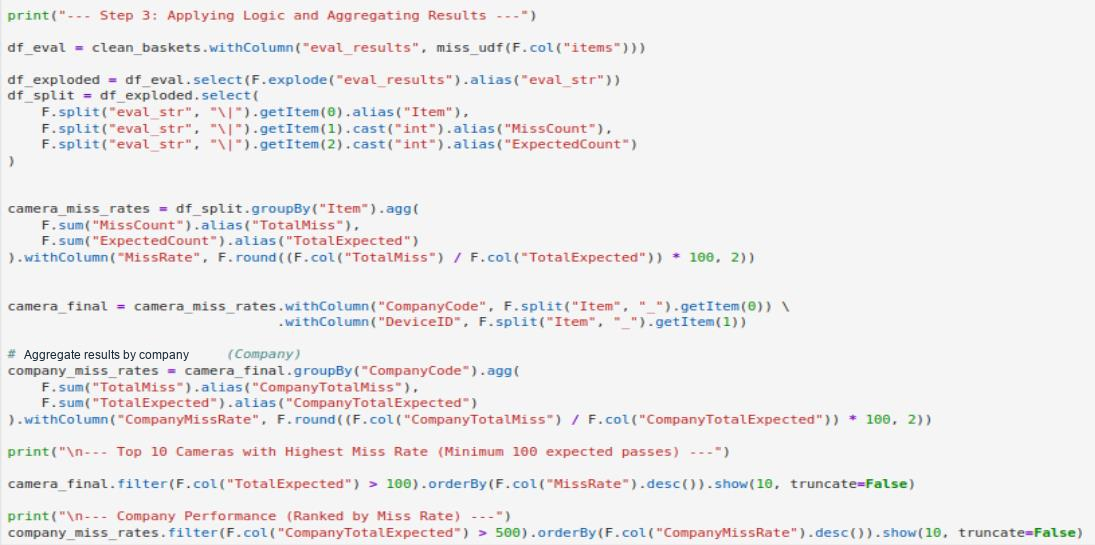
\includegraphics[width=\linewidth,height=.72\textheight,keepaspectratio]{assets/030_p010_02.png}\caption{Implementation and output: Frequent triples and algorithm choice.}\label{fig:030_p010_020}\end{figure}
\clearpage
\section{Camera and contractor miss heuristics}

The method broadcasts the top 50 frequent triples and examines baskets containing some expected items while lacking another. It interprets those partial sets as suspected missing registrations. The denominator is exposure inferred from patterns, not independently observed vehicles passing every camera. The narrative identifies camera 11238 of contractor 117 with a reported rate around 37.88 percent. Company-level examples include contractor 181 around 24.45 percent, 117 around 23.59 percent, and a comparison around 20.77 percent for 173 versus 23.87 percent for 123. Large exposure makes a moderate rate operationally consequential;\allowbreak{} the report mentions contractor 117 with over 1.5 million expected instances and more than 356,000 inferred misses. These are pattern-based flags. Alternate routes, missing observations elsewhere, window splitting, identifiers, and repeated exposure across triples can change rates. A partial basket does not prove a dirty lens, camera angle error, or ANPR failure. Operator aggregation should use explicit exposure weighting rather than an unweighted average of camera rates.

\begin{figure}[!htbp]\centering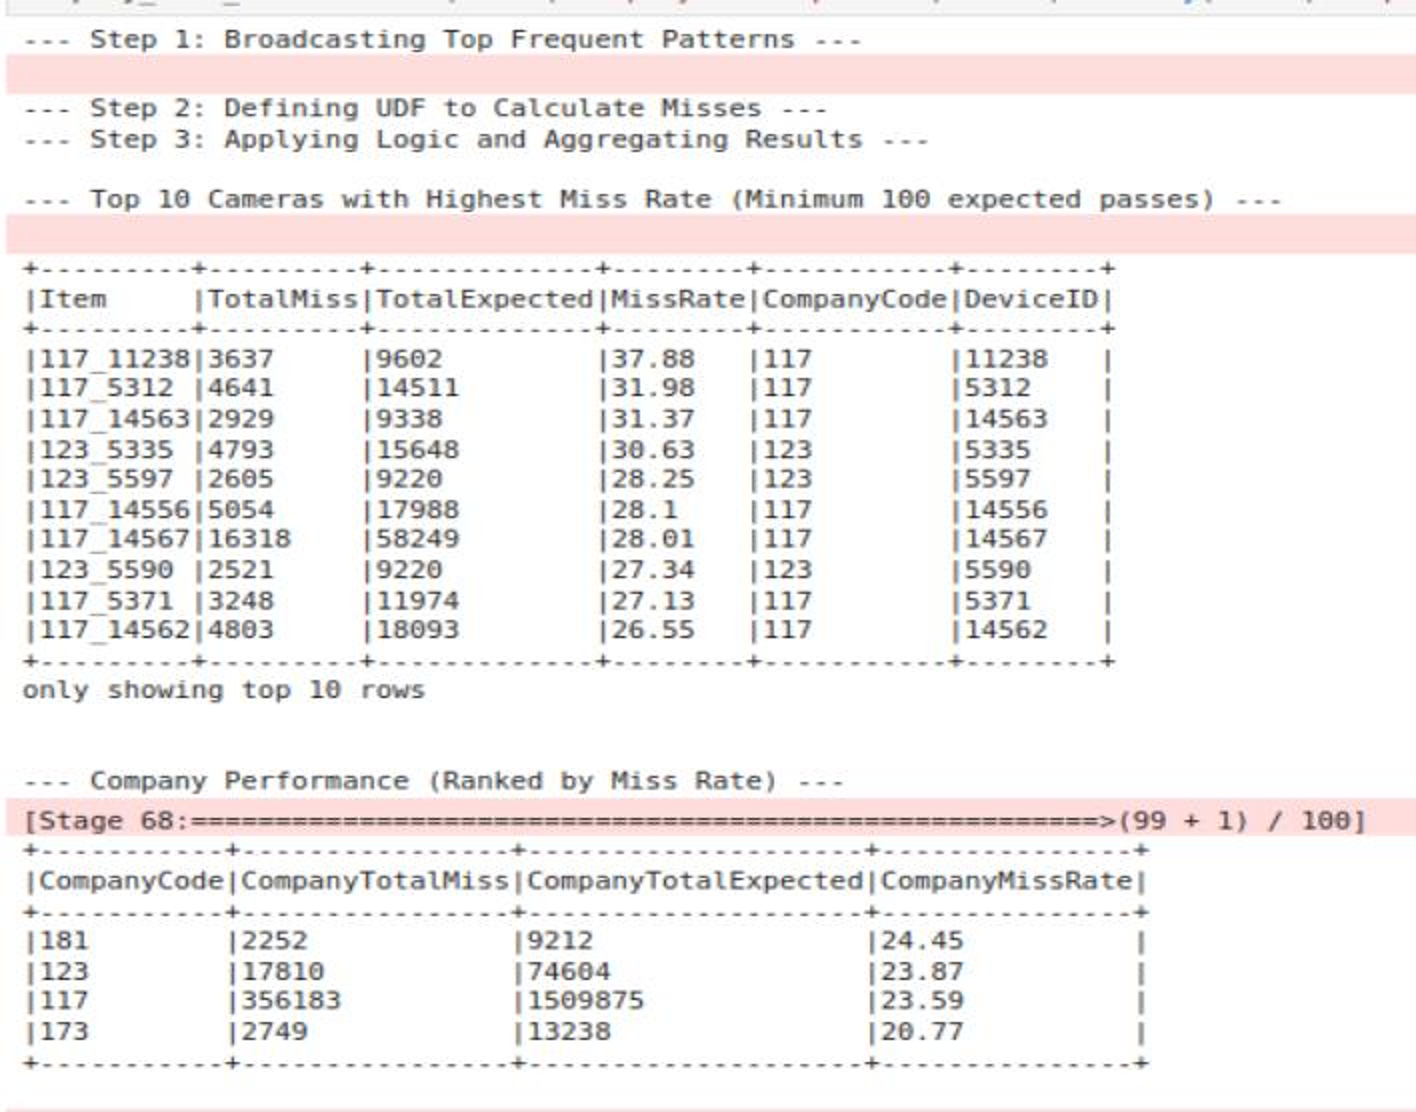
\includegraphics[width=\linewidth,height=.72\textheight,keepaspectratio]{assets/030_p011_01.png}\caption{Diagram or recorded result: Camera and contractor miss heuristics.}\label{fig:030_p011_010}\end{figure}
\begin{figure}[!htbp]\centering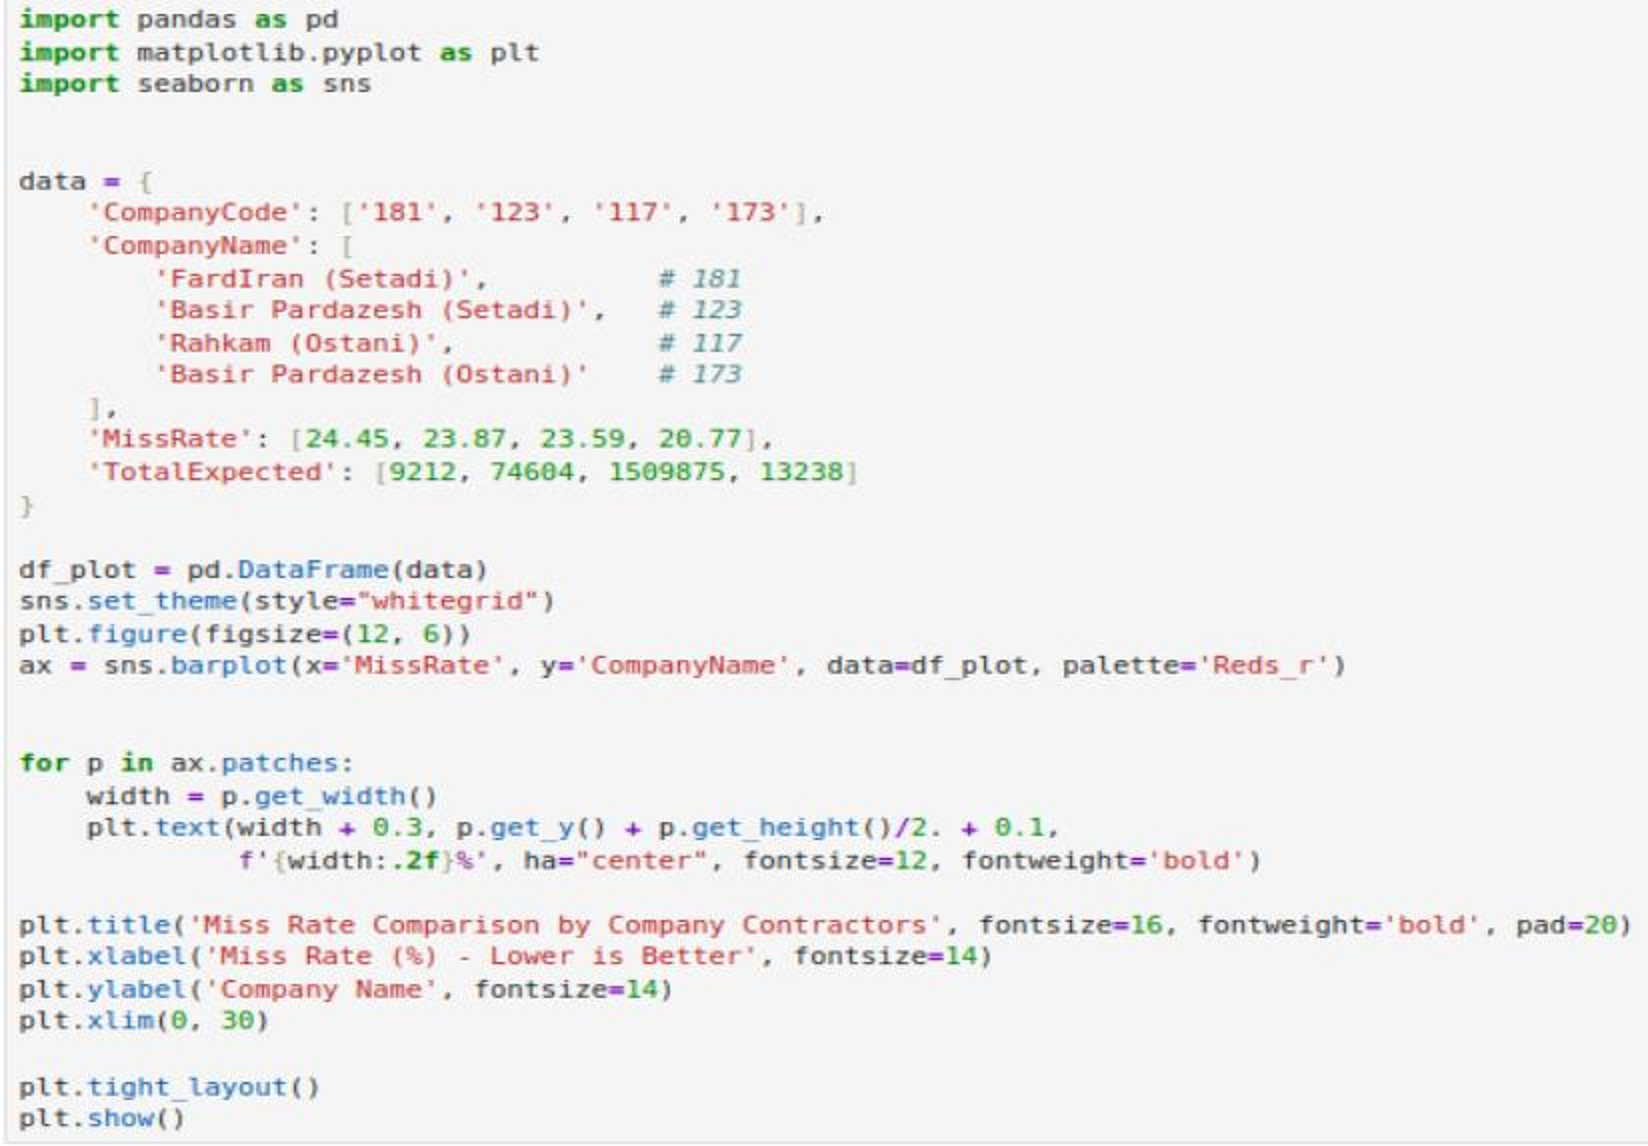
\includegraphics[width=\linewidth,height=.72\textheight,keepaspectratio]{assets/030_p011_02.png}\caption{Implementation and output: Camera and contractor miss heuristics.}\label{fig:030_p011_020}\end{figure}
\begin{figure}[!htbp]\centering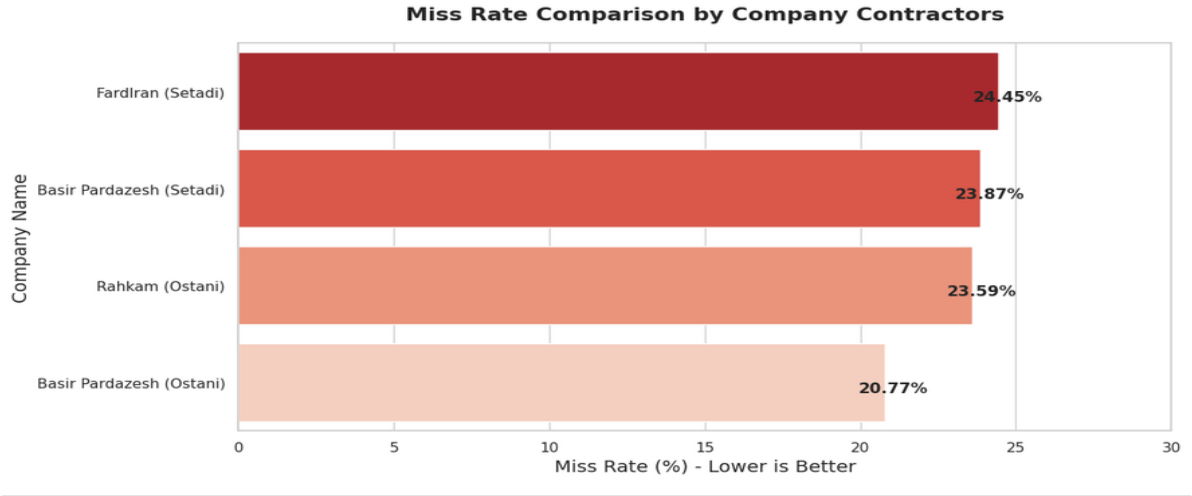
\includegraphics[width=\linewidth,height=.72\textheight,keepaspectratio]{assets/030_p012_01.png}\caption{Diagram or recorded result: Camera and contractor miss heuristics.}\label{fig:030_p012_010}\end{figure}
\clearpage
\section{MinHash/LSH route-set similarity}

Represent each vehicle by a set of road\_\allowbreak{}code values and use MinHash/\allowbreak{}LSH to produce candidates, with numHashTables=\allowbreak{}5 in the submitted Spark setup. Compute exact Jaccard on candidate sets. The report restricts execution to a random sample because of local resource limits and skew;\allowbreak{} therefore this is not a full-network all-pairs analysis. Pairs with Jaccard one have identical observed road sets, such as the displayed set containing 1338,1339,1012. They need not have the same order, direction, timestamp, or lane. Spark MinHashLSH's table parameter is not automatically a separately implemented textbook bands/\allowbreak{}rows design;\allowbreak{} document the actual API and candidate settings. Low route-set similarity can suggest that two vehicles have different observed coverage, but does not prove that a skipped camera is healthy. Perfect set similarity likewise does not prove an identical physical trip or eliminate all route confounders. LSH is approximate candidate generation and can omit similar pairs;\allowbreak{} exact Jaccard verifies only candidates considered.

\begin{figure}[!htbp]\centering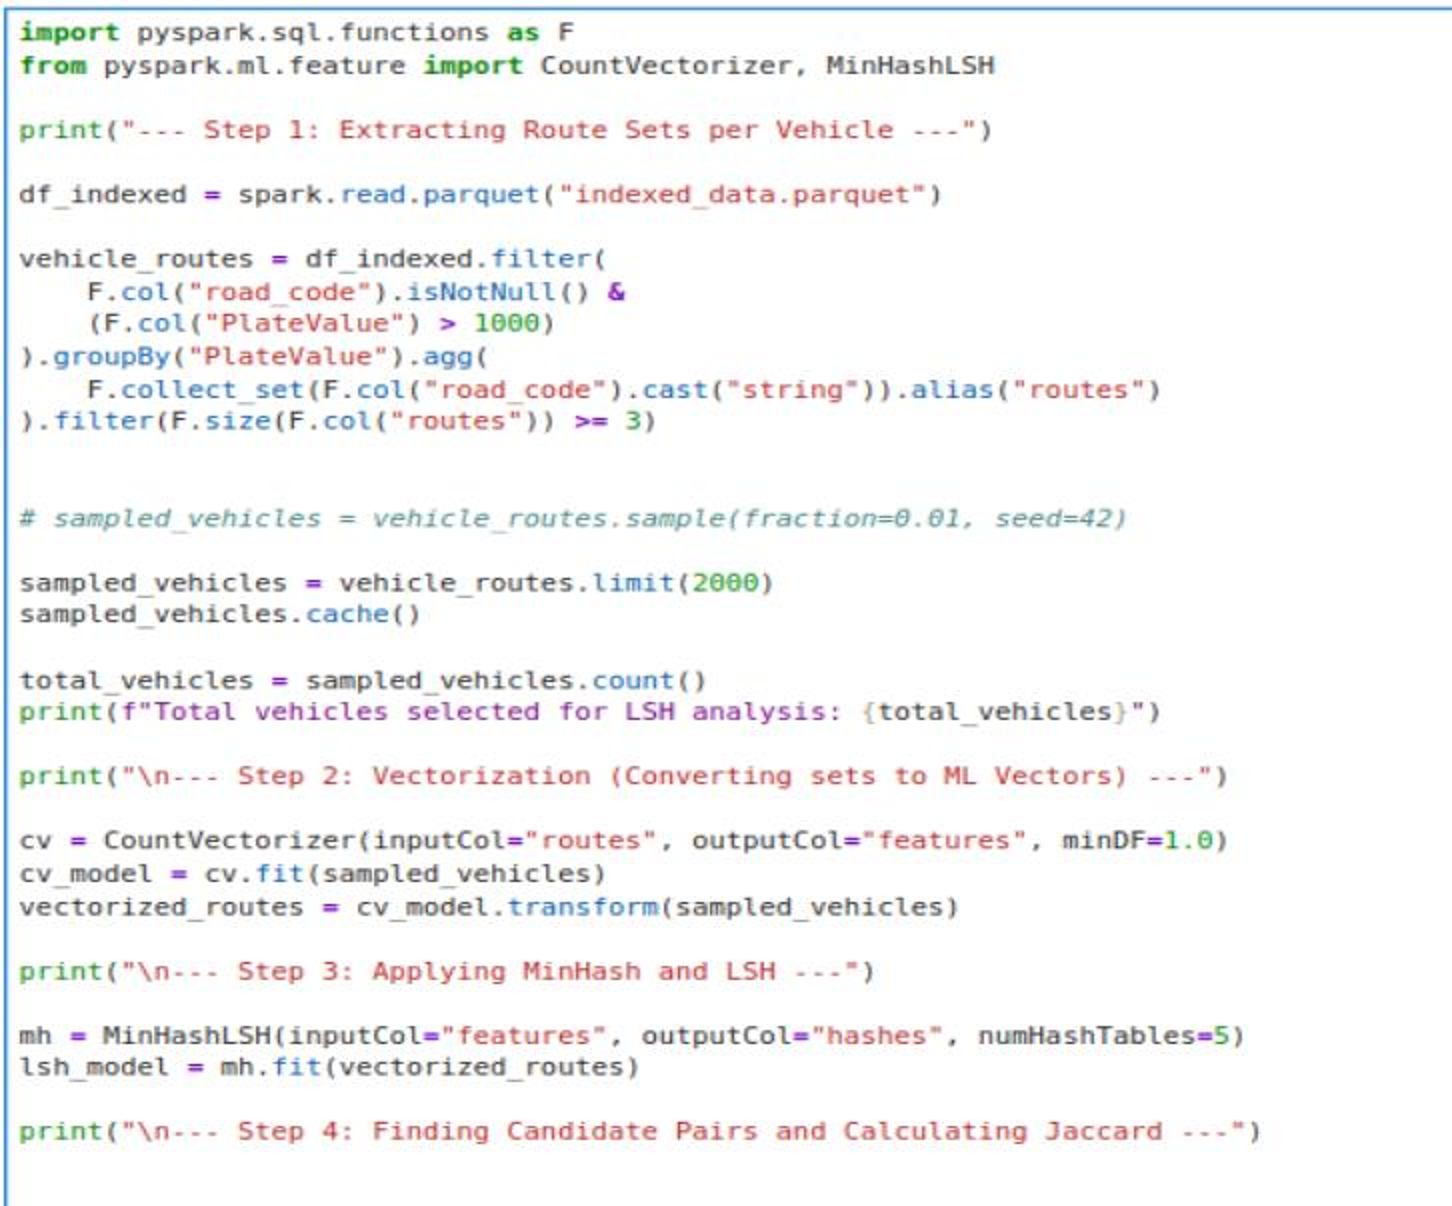
\includegraphics[width=\linewidth,height=.72\textheight,keepaspectratio]{assets/030_p014_01.png}\caption{Implementation and output: MinHash/LSH route-set similarity.}\label{fig:030_p014_010}\end{figure}
\begin{figure}[!htbp]\centering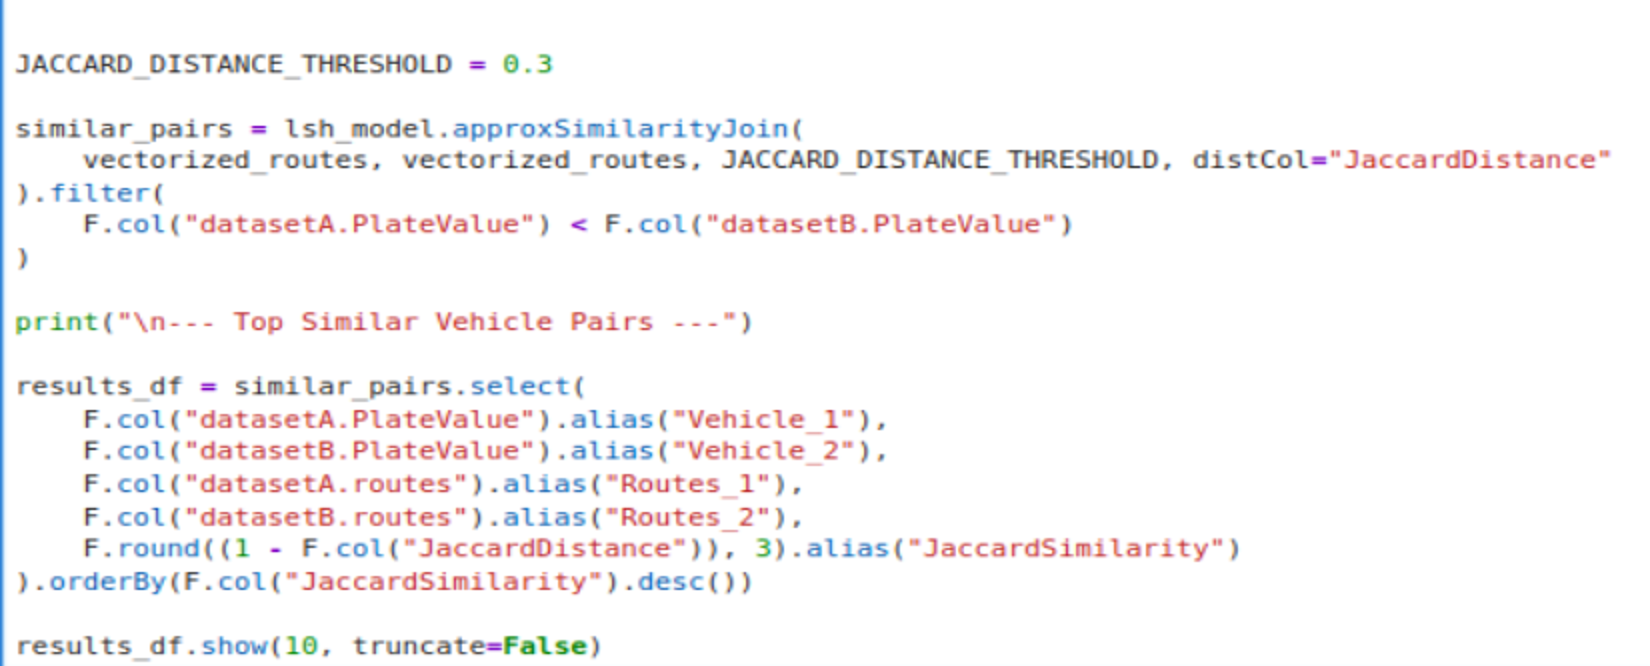
\includegraphics[width=\linewidth,height=.72\textheight,keepaspectratio]{assets/030_p014_02.png}\caption{Implementation and output: MinHash/LSH route-set similarity.}\label{fig:030_p014_020}\end{figure}
\begin{figure}[!htbp]\centering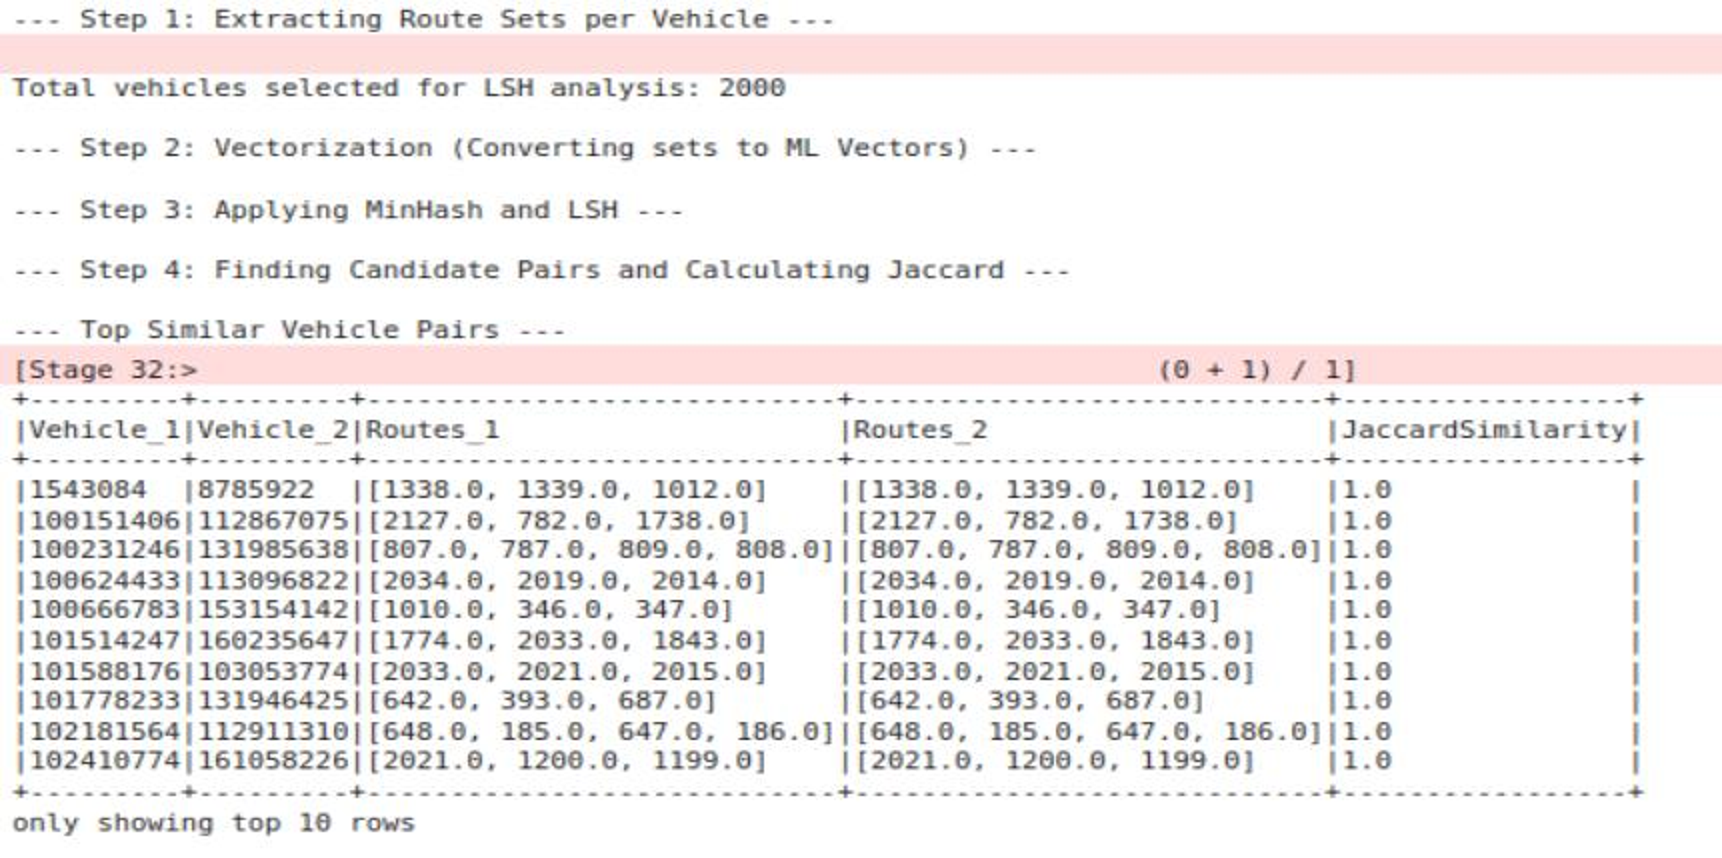
\includegraphics[width=\linewidth,height=.72\textheight,keepaspectratio]{assets/030_p014_03.png}\caption{Diagram or recorded result: MinHash/LSH route-set similarity.}\label{fig:030_p014_030}\end{figure}
\begin{figure}[!htbp]\centering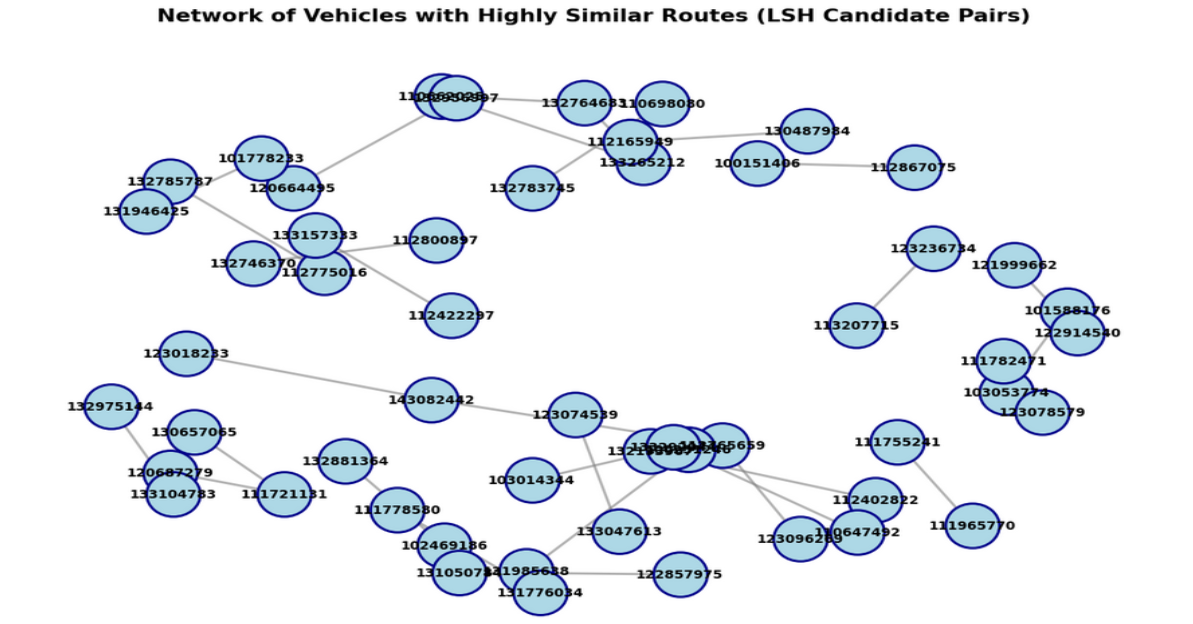
\includegraphics[width=\linewidth,height=.72\textheight,keepaspectratio]{assets/030_p016_01.png}\caption{Diagram or recorded result: MinHash/LSH route-set similarity.}\label{fig:030_p016_010}\end{figure}
\clearpage
\section{Engineering interpretation and preserved results}

The project joins data layout, basket mining, and route similarity into a framework for proposing quality checks. Its useful contribution is ranking suspicious patterns with clear evidence, not a validated hardware-failure classifier. Reproduction uses the notebook and dataset schema. Performance interpretation is limited to the recorded sample and execution environment.

\end{document}